\chapter{Clasificación de superficies compactas}

\section{Símplices}

\defn{Símplice}{
    Dados $k+1$ puntos $v_0,\dots,v_k\in\R^m$ afínmente independientes, el subconjunto convexo de $\R^m$ más pequeño que los contiene se conoce como un k-símplice y se denota por $\sigma = [v_0, \dots, v_k]$. Los puntos $v_i$ se llaman los vértices del k-símplice. Diremos que la dimensión de $\sigma$ es $k$.
}
\defn{Subsímplices, caras}{
    Si $\sigma=[v_0,\dots,v_k]$ es un k-símplice, cualquier subconjunto no vacío de vértices tambien determina un símplice que llamaremos subsímplice de $\sigma$. Si solo se omite un vértice, el subsímplice correspondiente se denomina una cara.
    \[\text{Las caras de }\sigma\text{ se denotan: } [v_0, \dots, \hat{v}_i, \dots, v_k], \text{ donde } \hat{v}_i \text{ es el vértice omitido.}\]
}

\ex{
    0-símplice (punto), 1-símplice (segmento de línea), 2-símplice (triángulo) y 3-símplice (tetraedro)
    \begin{center}
        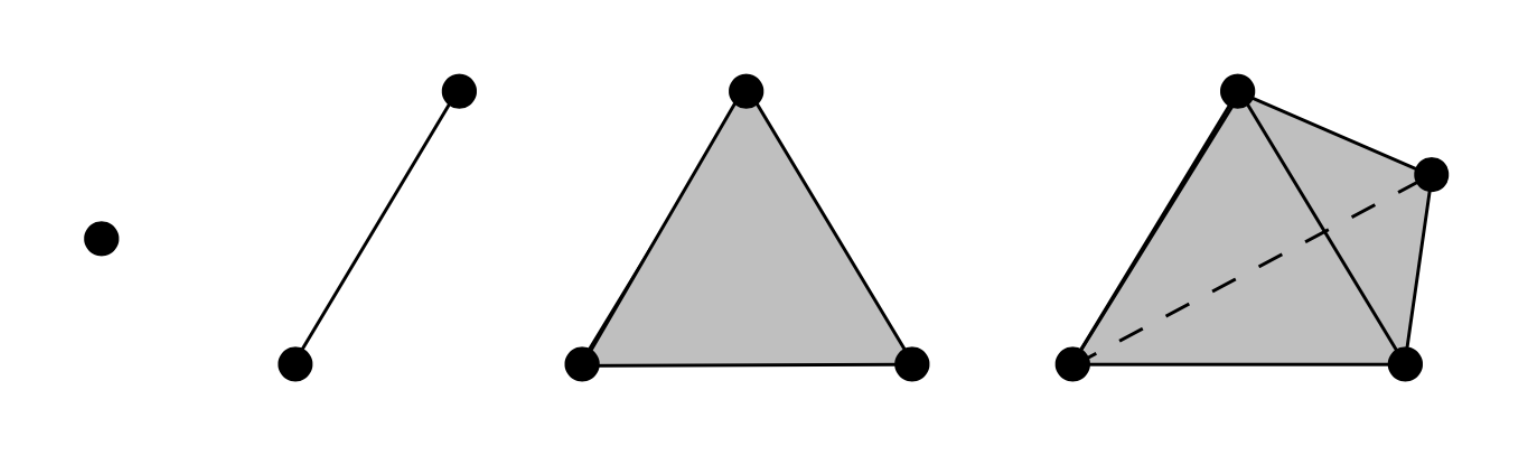
\includegraphics[width=0.7\linewidth]{img/ejemplos-simplices.png}
    \end{center}
}

\defn{Frontera}{
    Si $\sigma=[v_0,\dots,v_k]$ es un k-símplice, la unión de todas sus caras se denomina la frontera de $\sigma$ y se denota por 
    \[\partial\sigma = \displaystyle \bigcup_{0 \le i \le k}[v_0, \dots, \hat{v}_i, \dots, v_k].\]
}
\defn{Interior}{
    Si $\sigma$ es un k-símplice, el complementario de su frontera se denomina el interior de $\sigma$, 
    \[\text{int}(\sigma) = \sigma \setminus \partial\sigma\]
    Inmediatamente, se obtiene $\sigma = \text{int}(\sigma) \cup \partial\sigma$, donde la unión es disjunta.
}

\rmkb{
    La frontera y el interior de un k-símplice \(\sigma\) son conceptos independientes de la topología tomada sobre \(\R^m\). Sin embargo, si \(k = m\), entonces coinciden con la frontera y el interior topológicos de \(\sigma\) en topología usual de \(\R^m\).
}

\section{Complejos simpliciales}

\defn{Complejo simplicial}{
    Un complejo simplicial $K$ es una colección finita de símplices tal que:
    \begin{enumerate}
        \item Cada cara de cada símplice de $K$ también está en $K$.
        \item La intersección de cualesquiera dos símplices de $K$ es vacía o es un subsímplice de ambos.
    \end{enumerate}
    La dimensión de $K$ es la máxima dimensión de sus símplices.
}
\defn{Número de Euler}{
    Sea $K$ un complejo simplicial de dimensión n, si para cada $0 \le k \le n$ denotamos por $i_k$ el número de k-símplices de $K$, entonces el número (o característica) de Euler de $K$ es:
    \[\chi (K) = i_0 - i_1 + \dots + (-1)^n i_n.\]
}
\rmkb{
    Para el caso de un complejo simplicial de dimensión 2, denotando a los vértices $V = i_0$, aristas $E = i_1$ y caras $F=i_2$; la característica de Euler se puede expresar como:
    \[\chi = V - E + F\]
}
\defn{Poliedro asociado}{
    Dado un complejo simplicial $K$, la unión de todos los símplices de $K$ con la topología inducida por la topología usual de $\R^n$ se denomina el poliedro de $K$ y lo denotamos por $|K|$.
}

\section{Triangulaciones}

\defn{Triangulación}{
    Una triangulación de dimensión $n$ de un espacio topológico $X$ es un complejo simplicial $K$ de dimensión $n$ de forma que $|K|$ y $X$ son homeomorfos. En este caso se dice que $X$ es triangulable.
}

Enunciamos el siguiente teorema sin demostración:

\thmr{Teorema de Radó}{rado}{
    Toda superficie topológica admite una triangulación por un complejo simplicial de dimensión 2. Además cada 1-símplice (arista) es subsímplice de exactamente dos 2-símplices (cara).
}

\section{Presentación de superficies}

\defn{Letras y palabras}{
    Sea $A$ un conjunto finito (sus elementos los llamaremos letras). Una palabra $W$ es una sucesión finita de elementos de la forma $a$ ó $a^{-1}$, con $a \in A$, denotada por yuxtaposición.
}

\ex{
    Consideremos el conjunto $A=\{a,b,c\}$ formado por tres letras. Algunos ejemplos de palabras son los siguientes:
    \[W_1=cbab^{-1}ca^{-1},W_2=caab^{-1}bc^{-1},W_3=abb^{-1}a^{-1}.\]
}

\defn{Presentación poligonal}{
    Una presentación poligonal, escrita como $\partes =\langle A|W_1,\dots,W_k\rangle$, está formada por un conjunto finito de letras $A$ y una colección finita de palabras $W_1,\dots,W_k$ que cumplen:
    \begin{enumerate}
        \item Cada letra de $A$ aparece exactamente dos veces en todo el conjunto de palabras.
        \item Cada palabra tiene al menos longitud tres, salvo que haya una sola palabra que podría ser de dos letras.
    \end{enumerate}
}

\ex{
    Algunos ejemplos sencillos de presentaciones poligonales son los siguientes:
    \[\partes_1=\langle a\mid  aa^{-1}\rangle, \partes_2=\langle a,b\mid  aba^{-1}b^{-1}\rangle.\]

    \noindent Si consideramos el conjunto de letras y palabras del ejemplo anterior, $\partes=\langle A \mid W_1 \rangle$ es una representación poligonal, pero $\partes'=\langle A \mid W_3 \rangle$ no, ya que la letra $c$ no aparece exactamente dos veces en el conjunto de palabras.
}

\defn{Realización geométrica de $\partes$}{
    Toda presentación poligonal $\partes$ tiene asociado un espacio topológico $|\partes|$ (realización geométrica de $\partes$) construido como sigue: 
    \begin{enumerate}
        \item Para cada palabra se considera un polígono con el mismo número de aristas que la longitud de la palabra. 
        \item Cada arista se etiqueta correlativamente con las letras de la palabra y orientación opuesta si la letra está elevada a -1. 
        \item Finalmente, se identifican las aristas con el mismo nombre y orientación, mediante la topología cociente.
    \end{enumerate}
}

\clmp{}{$|\mathcal{P}|$ es un espacio topológico}{
    Pendiente.
}

\propp{Compacidad y conexión de $|\partes|$}{
    Dada una representación poligonal $\partes$, su realización geométrica, $|\partes|$, es una superficie compacta. Además si solo tiene una palabra, entonces es conexa.
}{
    Vamos a ver que el espacio topológico cociente $\tilde{X}$ es:
    \begin{enumerate}
        \item Compacto
        \item Superficie ($T_2$, $2A\N$, localmente euclídeo)
    \end{enumerate}

    \underline{Compacto:} Sea $X$ el polígono en $\R^2$, sea $\sim$ la relación de equivalencia entre las aristas y sea $\tilde{X}$ el cociente. X es compacto y $p : X \to \tilde{X}=\faktor{X}{\sim}$ la proyección al cociente es continua. Por tanto, $\tilde{X}$ es compacto.

    \underline{$T_2$:} Puedo tomar discos en $\R^2$ infinitamente pequeños de forma que separen los puntos en $X$ y las imágenes por $p$ separan los puntos de $\tilde{X}$.

    \underline{$2A\N$:} La proyección es continua, y el polígono es $2A\N$, luego $\tilde{X}$ también lo es.

    \underline{Localmente euclídeo:} La idea es distinguir 3 casos: 

    Veamos que $\faktor{\partes}{R}$ es localmente euclídeo. Necesitamos que para cada punto, haya un entorno que sea homeomorfo a un abierto de $\R^2$. 
    Sea $x \in \faktor{\partes}{R}$ y consideramos 
    \[\pi^{-1}(x) = \begin{cases}
        p \in \text{int}(\partes) \\
        \{q_1, q_2\} \in \text{aristas} \\
        \{v_1, \dots, v_k\} \in \text{vértices}
    \end{cases}\]
    \begin{enumerate}
        \item $\pi^{-1}(x) = p \in \text{int}(P)$. Entonces, $\pi|_{\text{int}(\partes)} : \text{int}(\partes) \to \pi(\text{int}(\partes))$ es biyectiva y continua y su inversa también es continua. Por tanto, como $\text{int}(\partes)$ es abierto, se tiene que es localmente euclídeo en $\text{int}(\partes)$.
        \item Tomamos $D_i \subset \R^2$ disco centrado en $q_i$ con $\overline{D_1} \cap \overline{D_2} = \emptyset$. Además, tampoco cortan ningun vértice de $\partes$.
        Sea $U_i = D_i \cap \partes \equiv$ semidiscos. Sea $h : a \to a'$ el homeomorfismo que da la relación de equivalencia (con $a, a'$ las aristas), es decir, $h(x)=y, x \in a, y \in a' \iff xRy$. 
        
        Existen homeomorfismos $\alpha_i : \R^2 \to \R^2$ (de hecho aplicaciones afines) tales que: 
        \[\alpha_1(U_1) = \{z\in \mathbb{C} : |z| < r_1, \text{Im}(z) \ge 0\} = \{(x,y)\in\R^2 : \|(x,y)\| < r_1, y \ge 0\}\]
        \[\alpha_2(U_2) = \{z\in \mathbb{C} : |z| < r_2, \text{Im}(z) \le 0\}\]
        y también que $\alpha_2 \circ h = \alpha_1|_a$.
        
        Sea $r = \min\{r_1, r_2\}$ y llamo $V_1 = \alpha^{-1}(\{z : |z|<r, \text{Im}(z) \ge 0\})$ y $V_2 = \alpha^{-1}(\{z : |z|<r, \text{Im}(z) \le 0\})$. Lo que hemos llamado $A = V_1 \cup V_2$ abierto de $\partes$. $\alpha : V_1 \cup V_2 \to B(0,r)$ identificación (continua, cerrada, sobreyectiva) donde $\alpha(x) = \begin{cases}
            \alpha_1(x) & x \in V_1 \\
            \alpha_2(x) & x \in V_2
        \end{cases}$. Está bien definida y pasa al cociente porque $xRy, x\in a, y \in a' \implies y = h(x)$ y entonces $\alpha(y) = \alpha_2(y) = \alpha_2(h(x)) = \alpha_1(x) = \alpha(x)$. % Falta la demostración visual, con los segmentos y los discos que se transforman en un circulito en R^2
        \item Sea ahora $\pi^{-1}(x) = \{v_1, \dots, v_k\}, k \in \N$. Consideramos $D_i$ disco infinitamente pequeño tal que $\overline{D_i} \cap \overline{D_j} = \emptyset, i \neq j$ no contenga puntos de otras aristas, ni vértices. 
        Sea $U_i = D_i \cap \partes \equiv$ sector circular. Supongamos los sectores ordenados de forma que $b_i \sim a_{i+1}, i=1,\dots,k$.

        Objetivo: $V_1 \cup \dots \cup V_k \overset{\alpha}{\longrightarrow} B(0,r) \subset \R^2$. 
        %TODO: No se hacer el dibujo este de la proyección canónica, ayuda!!

        Sea homeomorfismo afín $\alpha_i : \R^2 \to \R^2$ que lleva $U_i$ en $\{z : |z| < r_i, \text{arg}(z) \in [\frac{2\pi(i-1)}{k}, \frac{2\pi i}{k}]\}$ para todo $i=1,\dots,k$ cumpliendo $\alpha_{i+1} \circ h_i = \alpha_i|_{b_i}$, donde $h_i : b_i \to a_{i+1}$.
        
        Finalmente queda construir $\alpha_k : \R^2 \to \R^2$ que lleve $U_k$ en $\{z : |z| < r_k, \text{arg}(z) \in [\frac{2\pi(k-1)}{k}, 2\pi]\}$ y que cumpla 
        \begin{equation}
            \label{5.3-casos} \begin{cases}
                \alpha_k \circ h_{k-1} = \alpha_{k-1}|_{b_{k-1}} \\
                \alpha_1 \circ h_k = \alpha_k|_{b_k \equiv a_1}
            \end{cases}
        \end{equation}, con $h_k : b_k \to a_1$.
        
        Para garantizar la existencia de $\alpha_k$, podemos construirla en dos pasos, una para llevar a su hueco y otra para garantizar \ref{5.3-casos}. 

        Sea $r \le \min{r_1, \dots, r_k}$ y $V_i = \alpha_i^{-1}(\{z : |z| < r, \text{arg}(z) \in [\frac{2\pi(i-1)}{k}, \frac{2\pi i}{k}]\})$. Definimos $\alpha : V_1 \cup \dots \cup V_k \to B(0,r)$ como $\alpha(x) = \alpha_i(x), x \in V_i$. $\alpha$ está bien definida pues si $xRy, x\in b_i, y \in a_{i+1} \implies \alpha(y) = \alpha_{i+1}(h_i(x)) = \alpha_i(x) = \alpha(x), i\ne k$. Y para $k$, $y = h_k(x) \in a_1 \to$ misma cuenta. Luego, $\alpha$ es identificación (continua, sobreyectiva, cerrada) y $\tilde{\alpha}$ es homeomorfismo.
    \end{enumerate}
}

\defn{Presentación de una superficie compacta}{
    Sea $\mathcal{S}$ una superficie compacta. Una presentación de $\mathcal{S}$ es una presentación poligonal $\partes$ tal que $|\partes|$ y $\mathcal{S}$ son homeomorfas.
}

\propp{Presentación de $\mathcal{S}_1\#\mathcal{S}_2$}{
    Sean $\mathcal{S}_1$ y $\mathcal{S}_2$ dos superficies compactas y conexas presentadas por $\langle A_1|W_1 \rangle$ y $\langle A_2|W_2 \rangle$, respectivamente. Entonces, $\langle A_1 \sqcup A_2|W_1W_2 \rangle$ es una presentación de $\mathcal{S}_1\#\mathcal{S}_2$.
}{
    Sea $\partes_1$ polígono asociado a $W_1$ y sean $p,q \in \text{int}(\partes_1)$ dos puntos distintos y $v$ vértice de $partes_1$. 

    $\mathcal{S}_1 = \langle A_1|W_1 \rangle = \langle A_1 \sqcup {a,b,c}|W_1cba = Q_1, abc \rangle$. Definimos $\pi' : \partes_1 \sqcup Q_1 \to \mathcal{S}_1$ y $\pi:\partes_1 \to \mathcal{S}_1$. Sea entonces $B_1 = \pi'(\text{int}(Q_1)) \subset \mathcal{S}_1$. Si probamos que $B_1$ es homeomorfo a un disco, entonces tendremos que $\mathcal{S}_1\#\mathcal{S}_2$ se puede ver como $\mathcal{S}_1 \setminus Q_1 \sqcup \faktor{\mathcal{S}_2}{R_\varphi}$.

    Para ver que $B_1$ es homeomorfo a un disco, hacemos un razonamiento similar al de la proposición anterior tomando como abierto uno de la forma "sector circular" con $p$ y $q$ dentro del sector y $v$ el vértice, y hacer el mismo razonamiento con un solo sector.

    Así, tendremos que $\langle A_1 \sqcup \{a,b,c\}|W_1cba, a^{-1}b^{-1}c^{-1} \rangle$ es una presentación de $\mathcal{S}_1\setminus \text{int}(Q_1)$, análogamente $\langle A_2 \sqcup \{a',b',c'\}|W_2c'b'a', (a')^{-1}(b')^{-1}(c')^{-1} \rangle$ es presentación de $\mathcal{S}_2\setminus \text{int}(Q_2)$.

    Para obtener $\mathcal{S}_1\#\mathcal{S}_2$ identificamos $\varphi : \partial Q_1 \to \partial Q_2$, con $\varphi(a) = a', \varphi(b) = b', \varphi(c) = c'$ y obtenemos $\mathcal{S}_1\#\mathcal{S}_2 = \langle A_1 \sqcup A_2 \sqcup \{a,b,c\}|W_1cbaa^{-1}b^{-1}c^{-1}W_2\rangle = \langle A_1 \sqcup A_2|W_1W_2\rangle$.
}

\section{Teorema de Clasificación}

\defn{Transformaciones elementales sobre presentaciones poligonales}{
    Dada una presentación poligonal, llamaremos transformaciones elementales a las siguientes operaciones:
    \begin{itemize}
        \item \textbf{Renombrado:} Sustituir todas las apariciones de una letra $a$ por otra letra $b$ que no estuviera en la presentación.
        \item \textbf{Subdivisión:} Cambiar todas las apariciones de una letra $a$ por $ab$, y todas las apariciones de $a^{-1}$ por $b^{-1}a^{-1}$, donde $b$ es una letra nueva que no estaba en la presentación.
        \item \textbf{Consolidado: } Dadas dos letras $a$ y $b$ que siempre aparezcan juntas de la forma $ab$ o $b^{-1}a^{-1}$, sustituimos todas las apariciones de $ab$ por $c$, y todas las apariciones de $b^{-1}a^{-1}$ por $c^{-1}$, donde $c$ es una letra nueva que no estaba en la presentación.
        \item \textbf{Reflejo: } Cambiar una palabra de la forma $a_1a_2\dots a_k$ por $a_k^{-1}a_{k-1}^{-1}\dots a_1^{-1}$, donde $a_i$ son letras de la presentación.
        \item \textbf{Rotación: } Cambiar una palabra de la forma $a_1a_2\dots a_k$ por $a_2a_3\dots a_k a_1$, donde $a_i$ son letras de la presentación.
        \item \textbf{Corte:} Dada una palabra $W_1W_2$, con $W_1$ y $W_2$ no vacías, quitamos $W_1W_2$ de la presentación y añadimos $W_1a, a^{-1}W_2$ como palabras nuevas, donde $a$ es una letra nueva que no estaba en la presentación.
        \item \textbf{Pegado} Sustituimos dos palabras de la forma $W_1a, a^{-1}W_2$, con $W_1$ y $W_2$ arbitrarias y no vacías, por $W_1W_2$.
        \item \textbf{Plegado} Una palabra de la forma $W_1aa^{-1}$ se sustituye por $W_1$, donde $W_1$ tiene al menos longitud 3, salvo que haya una sola palabra, en cuyo caso podría ser de dos letras.
        \item \textbf{Desplegado} Una palabra de la forma $W_1$ se sustituye por $W_1aa^{-1}$, donde $W_1$ tiene al menos longitud 3, salvo que haya una sola palabra, en cuyo caso podría ser de dos letras.
    \end{itemize}
}

\defn{Presentaciones equivalentes}{
    Dos transformaciones poligonales se dice que son topológicamente equivalentes si sus realizaciones geométricas son homeomorfas.
}

\propp{Equivalencia por transformaciones elementales}{
    Cada una de las transformaciones elementales sobre una presentación poligonal produce otra presentación topológicamente equivalente. 
}{Pendiente.}

\lemp{Equivalencia entre algunos tipos de superficies}{
    \begin{enumerate}
        \item La botella de Klein y $\R\mathbb{P}^2\#\R\mathbb{P}^2$ son homeomorfas.
        \item $\mathbb{T}^2\#\R\mathbb{P}^2$ y $\R\mathbb{P}^2\#\R\mathbb{P}^2\#\R\mathbb{P}^2$ son homeomorfas.
    \end{enumerate}
}{
    El dibujo. 
}

\thm{Clasificación de superficies compactas}{
    Sea $S$ una superficie compacta y conexa, entonces $S$ es homeomorfa a una de las siguientes superficies:
    \begin{itemize}
        \item la esfera $\mathbb{S}^2$.
        \item una suma conexa de toros $\mathbb{T}^2\#\dots\#\mathbb{T}^2$.
        \item una suma conexa de planos proyectivos $\R\mathbb{P}^2\#\dots\#\R\mathbb{P}^2$.
    \end{itemize}
}
\pf{
    \noindent Sea $M$ una superficie compacta y conexa y sea $\partes$ una presentación poligonal. 

    \noindent \underline{Objetivo:} ver que $\partes$ es $\begin{cases}
        aa^{-1} \\
        a_1b_1a_1^{-1}b_1^{-1}\dots a_nb_na_n^{-1}b_n^{-1} \\
        a_1a_1\dots a_na_n         
    \end{cases}$

    \noindent Vamos a llamar aristas compementarias a aquellas que aparece como $a$ y $a^{-1}$. Aristas retorcidas las que aparecen como $a$ y $a$ ó $a^{-1}$ y $a^{-1}$.

    \noindent \underline{PASO 1:} Podemos suponer que $\partes$ tiene solo una palabra (o que el polígono tiene 1 sula cara). 
    Si dos palabras no tienen letras en común, entonces sus cocientes son disconexos (contradicción con que la superficie original es conexa (redactar mejor la contradicción si se quiere)). Y si tienen letras en común, rotando, reflejando y pegando podemos "unir" las palabras.

    \noindent Una cantidad finita de veces de este proceso demuestra el paso 1.

    \noindent \underline{PASO 2:} Podemos suponer que no hay pares de aristas complementarias adyacentes ($W_1aa^{-1}W_2$).
    Si las hubiera, plegando por ellas desaparecen. Excepto el caso en que solo tengamos ese par ($W_1, W_2 = \emptyset$). Pero entonces la superficie es una esfera.

    \noindent \underline{PASO 3:} Podemos suponer que todos los pares de aristas retorcidas son adyacentes ($VaWa$, con $V,W \ne \emptyset$). Cortamos por el medio ($Vab$ y $b^{-1}Wa$). Rotamos y pegamos por $a$ ($bVa$ y $a^{-1}W^{-1}b$). Entonces llegamos a $bbVW^{-1}$. 

    \noindent Una cantidad finita de este proceso demuestra el paso 3. 

    \noindent \underline{Nota:} Puede ser que tengamos que volver a aplicar el paso 2 ya que tenemos $W^{-1}$.

    \noindent \underline{PASO 4:} Podemos suponer que el polígono tiene todos sus vértices identificados.
    Sea $p:\partes \to M$ la proyección al cociente. Sea $p(v)=[v]$. Si todos los vértices no están identificados, existen vértices $v_1, w$ en $\partes$ y arista a ($v_1 \to w$) con $p(v_1)\ne p(w)$. La arista que termina en $v_1$ no puede ser ni $a$ (porque entonces $p(v_1) = p(w)$) ni $a^{-1}$ (por los pasos anteriores). Por tanto, la arista es distinta, la llamo $b$ y el otro vértice $x$, esto es que en $b$ tenemos ($x \to v_1$). 
    
    \noindent Suponemos que aparece $b^{-1}$ en otro sitio (si fuese $b$ sería análogo salvo una rotación en cierto momento). En ese $b^{-1}$ tendríamos ($v_1 \to x$). Tenemos entonces $baXb^{-1}Y$, con $X,Y \ne \emptyset$ (si no llegaríamos a alguna de estas igualdades: $p(v_1)=p(w)=p(x)$).
    
    \noindent Ahora cortamos por $c$ ($w \to x$). Rotando para pegar por $b$ (y reflejando si en vez de tener $b^{-1}$ tuvieramos $b$). Pegando llegamos a $acYc^{-1}X$, con ($v_1 \overset{a}{\to} w \overset{c}{\to} x \overset{Y}{\to} x \overset{c^{-1}}{\to} w \overset{X}{\to} v_1$).

    \noindent Por tanto, hemos reducido la cantidad de vértices que se identifican con $v$ en una unidad.

    \noindent Una cantidad finita de este proceso demuestra el paso 4.

    \noindent \underline{PASO 5:} Se cumple que si aparece un par $a, a^{-1}$, entonces hay otro par $b, b^{-1}$, es decir, de la forma $a\dots b\dots a^{-1} \dots b^{-1}$.

    \noindent Si no fuese así, tendría $aXa^{-1}Y$, donde $X$ e $Y$ no comparten letras o aristas (por los pasos anteriores). Esto significa que $X$ e $Y$ no comparten vértices (alguna de las aristas que sale de ese vértice tendria que estar "allí"), es decir, que los vértices finales de $a$ y $a^{-1}$ que solo tocan $X$ solo pueden identificarse con vértices de $X$, y los iniciales solo pueden con $Y$.

    \noindent Como cualquier arista $c \subset X$ cumple que su identificación tambien está contenida en $X$, entonces todos los vértices que se identifican con $X$ están en $X$. Si otro vértice se identificara con $x$ y estuviese en $Y$, habría una arista a la vez en $X$ e $Y$. Por tanto, tendríamos dos clases de vértices distintos $p(x) \ne p(y)$, que es una contradicción con el hecho de que todos los vértices estaban \textcolor{red}{BLANK} (no lo he escuchado, lo siento).

    \noindent \textcolor{red}{!ATENCIÓN!} El dibujo que hizo en clase con las $c$'s es muy instructivo para ver esto. Si alguien lo tiene copiado y lo pone como imagen sería maravilloso (una imagen vale más que mil palabras).

    \noindent \underline{PASO 6:} Podemos suponer que los pares de aristas del paso 5 aparecen consecutivos. 

    \noindent $aXbYa^{-1}Zb^{-1}W$. Cortamos desde el final de $X$ al final de $W$, y llamamos a esa arista $c$. Vamos a pegar por $a$. Tendremos $aXcW$ y $bYa^{-1}Zb^{-1}c^{-1}$. Rotando de buena manera y pegando se queda $YXcWzb^{-1}c^{-1}b$. Ahora cortamos desde el final de $b^{-1}$ al final de $c$, llamando $d$ a esa arista. Se nos queda $YXcd^{-1}c^{-1}b$ y $WZb^{-1}d$. Rotando y pegando por $b$ se nos queda $YXcd^{-1}c^{-1}dWZ$. 

    \noindent Una cantidad finita de este proceso demuestra el paso 6.

    \noindent \underline{PASO 7:} Aplicar $\mathbb{T}^2\#\R \mathbb{P}^2$ y $\R \mathbb{P}^2\#\R \mathbb{P}^2\#\R \mathbb{P}^2$.
}